\documentclass[tikz,border=5mm]{standalone}
\usepackage{tikz}
\usetikzlibrary{shapes.geometric,arrows.meta,positioning,fit,backgrounds,calc}
\usepackage{amsmath}

\newcommand{\cmark}[1]{\raisebox{.5pt}{\textcircled{\raisebox{-.9pt}{\scriptsize\bfseries #1}}}}

% ── Colors ──
\definecolor{cBlue}{RGB}{66,133,244}
\definecolor{cBlueFill}{RGB}{215,232,255}
\definecolor{cOrange}{RGB}{230,162,60}
\definecolor{cOrangeFill}{RGB}{255,240,218}
\definecolor{cGreen}{RGB}{76,175,80}
\definecolor{cGreenFill}{RGB}{225,245,228}
\definecolor{cRed}{RGB}{211,84,85}
\definecolor{cRedFill}{RGB}{255,232,234}
\definecolor{cPurple}{RGB}{126,87,194}
\definecolor{cPurpleFill}{RGB}{237,231,246}
\definecolor{cTeal}{RGB}{0,151,167}
\definecolor{cTealFill}{RGB}{220,246,249}
\definecolor{cYellow}{RGB}{245,166,35}
\definecolor{cYellowFill}{RGB}{255,247,220}
\definecolor{cDarkRed}{RGB}{183,28,28}
\definecolor{cDarkGreen}{RGB}{46,125,50}

\tikzset{
    box/.style={rectangle, rounded corners=4pt, thick,
        minimum height=1.1cm, font=\large, align=center},
    sbox/.style={rectangle, rounded corners=3pt, semithick,
        minimum height=0.9cm, font=\normalsize, align=center},
    client/.style={box, draw=cBlue, fill=cBlueFill, minimum width=2.0cm,
        font=\normalsize},
    server/.style={box, draw=cOrange, fill=cOrangeFill, very thick,
        minimum width=3.0cm, minimum height=1.2cm, font=\large},
    dtmod/.style={sbox, draw=cGreen, fill=cGreenFill, minimum width=3.2cm},
    gen/.style={sbox, draw=cTeal, fill=cTealFill, minimum width=3.2cm},
    verify/.style={box, draw=cRed, fill=cRedFill, minimum width=3.2cm,
        minimum height=2.0cm},
    dtpw/.style={box, draw=cPurple, fill=cPurpleFill, minimum width=3.2cm,
        minimum height=2.0cm},
    agg/.style={box, draw=cYellow, fill=cYellowFill, very thick,
        minimum width=3.2cm},
    gate/.style={diamond, draw=black!70, fill=white, thick,
        minimum width=1.2cm, minimum height=1.2cm,
        font=\normalsize\bfseries, aspect=2.2, inner sep=1pt},
    arr/.style={-{Stealth[length=3.5mm,width=3mm]}, thick, #1},
    arr/.default={black!60},
    darr/.style={-{Stealth[length=3.5mm,width=3mm]}, thick, dashed, #1},
    darr/.default={black!40},
    lbl/.style={font=\normalsize, fill=white, inner sep=2pt,
        rounded corners=1pt},
}

\begin{document}
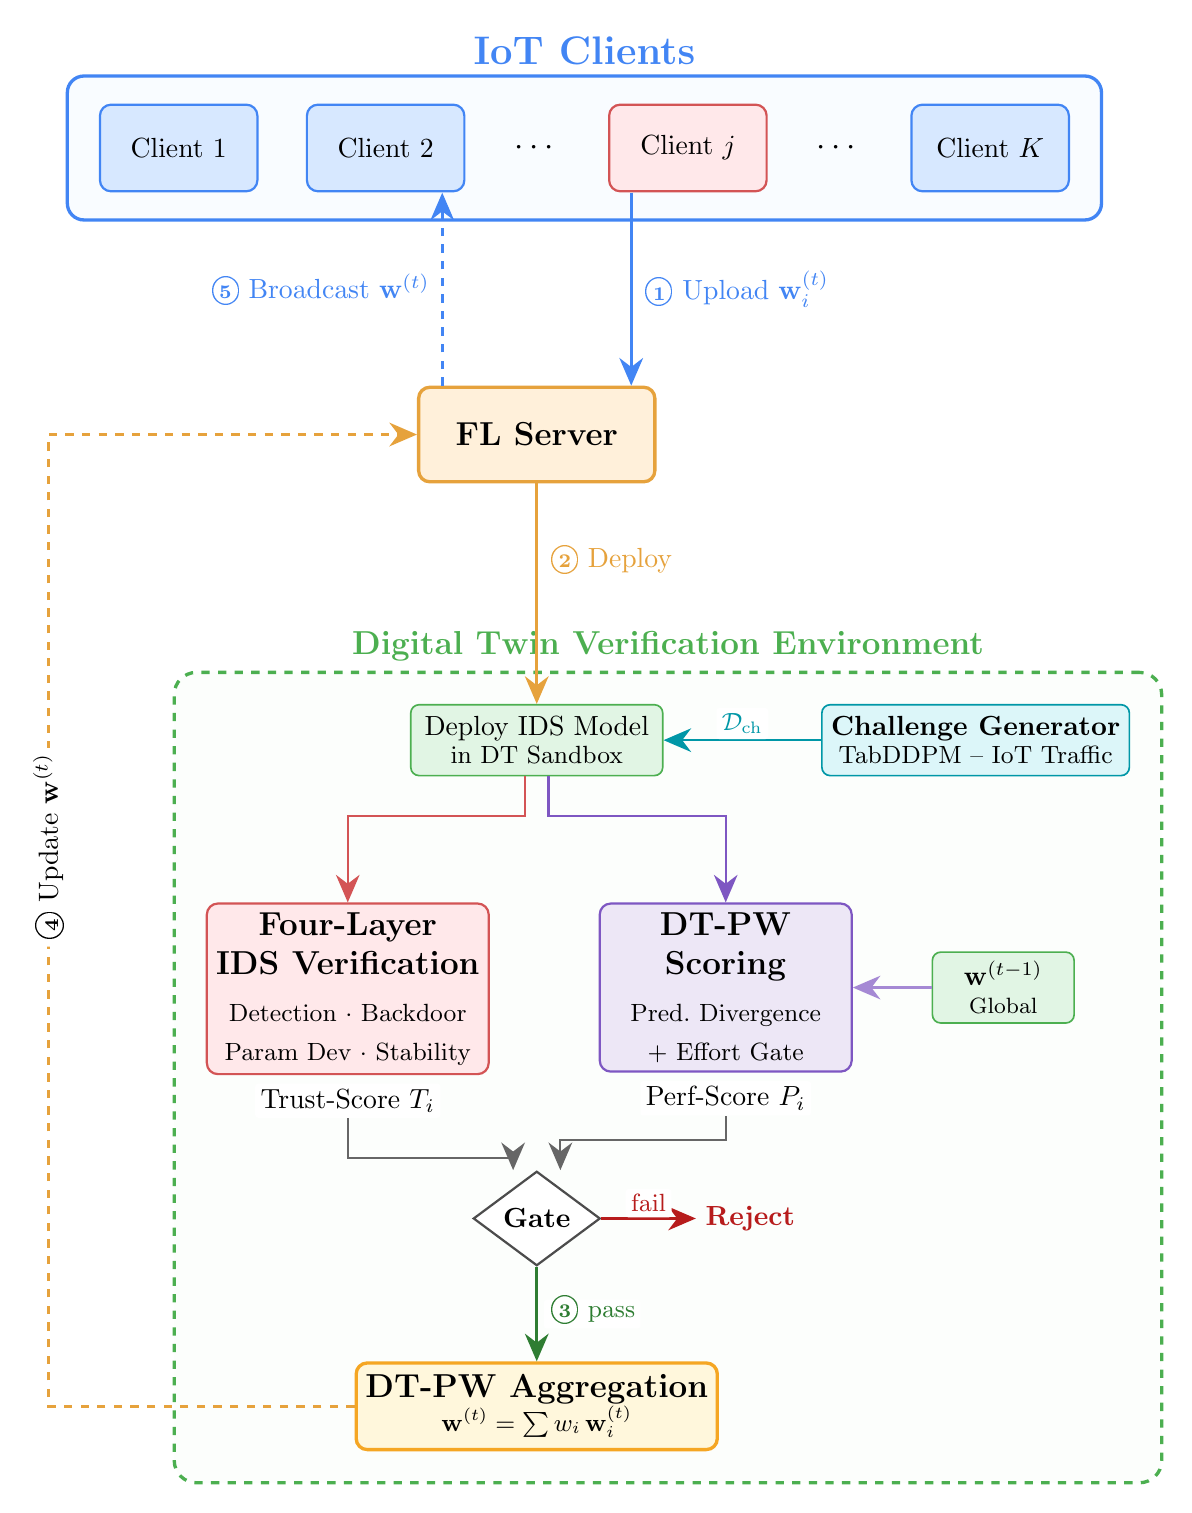
\begin{tikzpicture}[node distance=0.8cm and 1.0cm]

% ================================================================
%  TOP — IoT Clients (horizontal row inside a box)
% ================================================================
\node[client] (c1) {Client 1};
\node[client, right=0.6cm of c1] (c2) {Client 2};
\node[font=\large, right=0.5cm of c2] (cdots) {$\cdots$};
\node[client, right=0.5cm of cdots, draw=cRed, fill=cRedFill] (cj) {Client $j$};
\node[font=\large, right=0.5cm of cj] (cdots2) {$\cdots$};
\node[client, right=0.5cm of cdots2] (ck) {Client $K$};

% Invisible anchor for clientbox (drawn on background so client fills show)
\coordinate (cbl) at ($(c1.north west)+(-0.4,0.35)$);
\coordinate (cbr) at ($(ck.south east)+(0.4,-0.35)$);

% ================================================================
%  FL Server (below clients, centered)
% ================================================================
\node[server, below=2.5cm of cdots, yshift=-0.3cm] (srv) {\textbf{FL Server}};

% ── Upload: clientbox → server (right side) ──
\draw[arr=cBlue, very thick]
    ($(cdots.south)+(1.2,-0.35)$) -- ($(srv.north)+(1.2,0)$)
    node[lbl, pos=0.5, right, xshift=2pt] {\cmark{1}\;Upload $\mathbf{w}_i^{(t)}$};

% ── Broadcast: server → clientbox (left side) ──
\draw[darr=cBlue, very thick]
    ($(srv.north)+(-1.2,0)$) -- ($(cdots.south)+(-1.2,-0.35)$)
    node[lbl, pos=0.5, left, xshift=-2pt] {\cmark{5}\;Broadcast $\mathbf{w}^{(t)}$};

% ================================================================
%  DIGITAL TWIN — below server (more spacing to avoid label overlap)
% ================================================================

% Deploy box
\node[dtmod, below=2.8cm of srv, font=\normalsize] (deploy)
    {Deploy IDS Model\\[-2pt]{\small in DT Sandbox}};

% Arrow: server → deploy
\draw[arr=cOrange, very thick] (srv.south) --
    node[lbl, right, xshift=2pt, pos=0.35] {\cmark{2}\;Deploy} (deploy.north);

% Challenge Generator (to the right of deploy)
\node[gen, right=2.0cm of deploy] (genr)
    {\textbf{Challenge Generator}\\[-2pt]{\small TabDDPM -- IoT Traffic}};

% Arrow: generator → deploy
\draw[arr=cTeal] (genr.west) --
    node[lbl, above] {\small $\mathcal{D}_{\text{ch}}$} (deploy.east);

% ── Two parallel branches below deploy ──

% LEFT branch: Four-Layer Pipeline
\node[verify, below=1.6cm of deploy, xshift=-2.4cm] (pipe) {
    \textbf{Four-Layer}\\
    \textbf{IDS Verification}\\[3pt]
    {\small Detection $\cdot$ Backdoor}\\
    {\small Param Dev $\cdot$ Stability}
};

% RIGHT branch: DT-PW Scoring
\node[dtpw, below=1.6cm of deploy, xshift=2.4cm] (pw) {
    \textbf{DT-PW}\\
    \textbf{Scoring}\\[3pt]
    {\small Pred.\ Divergence}\\
    {\small + Effort Gate}
};

% Global model reference → DT-PW (straight horizontal arrow)
\node[sbox, draw=cGreen, fill=cGreenFill, minimum width=1.8cm,
      right=1.0cm of pw, font=\normalsize] (gm)
    {$\mathbf{w}^{(t-1)}$\\[-2pt]{\footnotesize Global}};
\draw[arr=cPurple!70] (gm.west) -- (pw.east);

% Arrows: deploy → branches
\draw[arr=cRed]    ($(deploy.south)+(-0.15,0)$) -- ++(0,-0.5) -| (pipe.north);
\draw[arr=cPurple] ($(deploy.south)+(+0.15,0)$) -- ++(0,-0.5) -| (pw.north);

% Score output labels
\node[lbl, below=0.1cm of pipe, font=\normalsize] (tlbl) {Trust-Score $T_i$};
\node[lbl, below=0.1cm of pw, font=\normalsize]   (plbl) {Perf-Score $P_i$};

% ================================================================
%  BOTTOM — Decision Gate + Aggregation
% ================================================================
\node[gate, below=1.8cm of deploy, yshift=-3.2cm] (gate) {Gate};

% Trust-Score → Gate
\draw[arr] (tlbl.south) -- ++(0,-0.5) -| ($(gate.north)+(-0.3,0)$);
% Perf-Score → Gate
\draw[arr] (plbl.south) -- ++(0,-0.3) -| ($(gate.north)+(+0.3,0)$);

% Reject (to the right of gate)
\node[font=\normalsize\bfseries\color{cDarkRed}, right=1.2cm of gate] (rej) {Reject};
\draw[arr=cDarkRed] (gate.east) -- node[lbl, above] {\small fail} (rej.west);

% Aggregation (below gate)
\node[agg, below=1.2cm of gate, font=\large] (agg)
    {\textbf{DT-PW Aggregation}\\[-2pt]
     {\small $\mathbf{w}^{(t)} = \sum w_i\,\mathbf{w}_i^{(t)}$}};
\draw[arr=cDarkGreen, very thick] (gate.south) --
    node[lbl, right, xshift=2pt] {\cmark{3}\;\small pass} (agg.north);

% ================================================================
%  FEEDBACK — Aggregation back to server (far left, outside DT box)
% ================================================================
\coordinate (fb_left) at ($(pipe.west)+(-2.0,0)$);
\coordinate (fb_top)  at (fb_left |- srv.west);
\draw[darr=cOrange, very thick]
    (agg.west) -- ++(0,0) -| (fb_left) -- (fb_top) -- (srv.west);
\node[lbl, rotate=90] at ($(fb_left)!0.45!(fb_top)$) [left, xshift=-3pt]
    {\cmark{4}\;Update $\mathbf{w}^{(t)}$};

% ================================================================
%  BACKGROUND REGIONS (drawn behind everything)
% ================================================================
\begin{scope}[on background layer]

    % IoT Clients box (background so client fills render on top)
    \node[draw=cBlue, very thick, rounded corners=6pt, fill=cBlueFill!15,
          fit=(c1)(c2)(cdots)(cj)(cdots2)(ck),
          inner xsep=0.4cm, inner ysep=0.35cm,
          label={[font=\Large\bfseries\color{cBlue}]above:IoT Clients}] (clientbox) {};

    % Digital Twin environment (label above the border, not inside)
    \node[draw=cGreen, very thick, dashed, rounded corners=8pt,
          fill=cGreenFill!10,
          fit=(genr)(deploy)(pipe)(pw)(gm)(tlbl)(plbl)(gate)(agg)(rej),
          inner xsep=0.4cm, inner ysep=0.4cm,
          label={[font=\large\bfseries\color{cGreen}]%
                 above:Digital Twin Verification Environment}] {};
\end{scope}


\end{tikzpicture}
\end{document}
